\documentclass[10pt]{article}

\usepackage[T1]{fontenc}
\usepackage{lmodern}
\usepackage[letterpaper,left=0.78in,right=0.78in,top=0.70in,bottom=0.70in]{geometry}
\usepackage{microtype}
\usepackage{graphicx}
\usepackage{booktabs}
\usepackage{xcolor}
\usepackage{float}
\usepackage[
  colorlinks=true,
  linkcolor=MolariumBlue,
  citecolor=MolariumBlue,
  urlcolor=MolariumBlue,
  pdftitle={Molecular design software is now free: building a browser molecular workbench with GPT-5.6 Sol},
  pdfauthor={Rafal P. Wiewiora and Woody Sherman}
]{hyperref}

\definecolor{MolariumBlue}{HTML}{245A78}
\definecolor{MolariumGreen}{HTML}{2F8067}
\definecolor{MolariumMint}{HTML}{EDF7F3}
\setlength{\parindent}{1.15em}
\setlength{\parskip}{0.12em}
\setlength{\textfloatsep}{0.65em}
\setlength{\floatsep}{0.55em}
\setlength{\abovecaptionskip}{0.38em}
\setlength{\belowcaptionskip}{0pt}
\setlength{\emergencystretch}{2em}
\renewcommand{\arraystretch}{1.08}
\newcommand{\molarium}{\textsc{Molarium}}
\newcommand{\claimbox}[1]{%
  \par\smallskip\noindent
  \fcolorbox{MolariumGreen}{MolariumMint}{%
    \parbox{0.955\linewidth}{\centering\bfseries\color{MolariumGreen}#1}}%
  \par\smallskip}

\begin{document}
\begin{center}
\vspace*{-1.3em}
{\LARGE\bfseries Molecular design software is now free}\\[0.18em]
{\large Building a browser molecular workbench with GPT-5.6 Sol}\\[0.48em]
{\normalsize Rafal P. Wiewiora \quad Woody Sherman}\\[0.18em]
{\small PsiThera, Watertown, MA}\\[0.32em]
\href{https://molarium.org}{molarium.org} \quad August 2026
\end{center}
\vspace{0.2em}

\begin{abstract}
\noindent
What happens when a chemist asks a coding agent for the molecular-design
environment they actually want, then refuses to accept toy chemistry? Over
several days, that conversation produced \molarium{}: a public browser
workbench for three-dimensional editing, protein preparation, conformer search,
molecular mechanics, ANI-2x, and short-chain protein prediction. GPT-5.6 Sol did
not merely connect existing commands. It wrote browser-native Sage forces,
OBC2/ACE solvent, SHAKE/RATTLE constraints, a homogeneous-replica molecular
dynamics engine, and ANI-2x descriptor and force kernels. We tested those parts
against OpenMM, TorchANI, finite differences, and fixed fixtures. The artifact
is therefore more than another software release. It is evidence that, under
expert direction, a current model can turn published methods into substantial,
inspectable scientific code while the research conversation is still under
way. Equations and parameters made the new implementations testable; trained
weights and accumulated validation still had to be preserved and reused.
\end{abstract}

\claimbox{The result is not merely that an agent can operate scientific
software. A chemist asked for missing software, tested it while it was being
written, and kept the resulting methods as inspectable code.}

\section{A molecule should not disappear into its software}

Molecular design begins with an act of spatial imagination: a chemist sees a
molecule that does not yet exist. It is a beautiful job, and its software should
honor it. Instead, the idea is often broken into a drawing package, a preparation
wizard, a simulation script, a queue, and a different viewer for the answer.
Each handoff asks the chemist to remember what the software has forgotten. The
tools become the work.

We wanted the opposite feeling: the quiet pleasure of software that simply
works. The molecule should turn when the chemist turns it. A carbonyl-to-enol
edit should remain in front of them until both bond-order changes are finished.
A calculation should return to the same scene, not to an anonymous output
directory. The machinery should recede so that attention can stay with shape,
strain, water, and the next chemical idea.

\paragraph{Why the browser, and why now.}
For many years the browser was mainly a viewer or a front end to a remote
calculation. Two platform changes made a local scientific application plausible.
WebAssembly provided a portable, sandboxed target for mature C and C++
libraries, avoiding a complete rewrite in JavaScript~\cite{webassembly}. WebGPU
then exposed modern GPU buffers, compute shaders, and command queues through one
browser API backed by native graphics systems~\cite{webgpu}. Web molecular
graphics had already established the interactive side of the problem
\cite{ngl}. The remaining step was to place chemical perception, numerical
kernels, and the molecular canvas in the same local runtime.

This division suits molecular design. WebAssembly handles graph operations,
file formats, control flow, and reference calculations. WebGPU handles repeated
floating-point work across atoms or conformers. Workers keep long calculations
off the interface thread. The application can be served as static files, while
the structures and supported calculations remain on the user's device. OpenMM
also provides an independent reference against which narrower browser kernels
can be tested~\cite{openmm8}.

The more provocative result is not the interface but how it appeared. The first
instruction was almost unserious: build a copy of an existing molecular viewer.
Minutes later the first benzene was visibly wrong. ``Can you actually test all
this out?'' became the governing question. A methyl fragment made a false bond;
a trifluoromethyl group arrived flat; changing one bond order prematurely bent
an oxygen and rotated a ligand. Each visual objection became a test and then a
change in the model of the molecule. Bond perception was separated from drawing;
fragments received three-dimensional starting conformations; coupled edits were
staged; cleanup was restricted to the atoms near the change.

The same pattern drove the numerics. ``Is this a real force field?'' killed an
early toy evaluator and moved the project to RDKit MMFF/UFF and prepared OpenFF
Sage Systems~\cite{rdkit,mmff94,uff,sage}. A disagreement between CPU and GPU energies exposed both a unit
mistake and an architectural misunderstanding: OpenMM Reference in WebAssembly
was a CPU oracle, not the WebGPU engine. ``Wait---aren't we using WebGPU?'' led
to analytic WGSL forces, then compact sparse buffers, then tests on Trp-cage and
ubiquitin. Asking for implicit solvent led to OBC2/ACE~\cite{obc2,ace}; asking whether that
included SHAKE led to fixed-point SHAKE/RATTLE~\cite{shake,rattle}; a 100,000-step run that stopped
immediately exposed a forgotten 5,000-step validation cap. This was not a model
producing a finished application from one prompt. It was a chemist noticing the
wrong thing on screen and an agent turning that objection into code, repeatedly.

\begin{figure}[H]
  \centering
  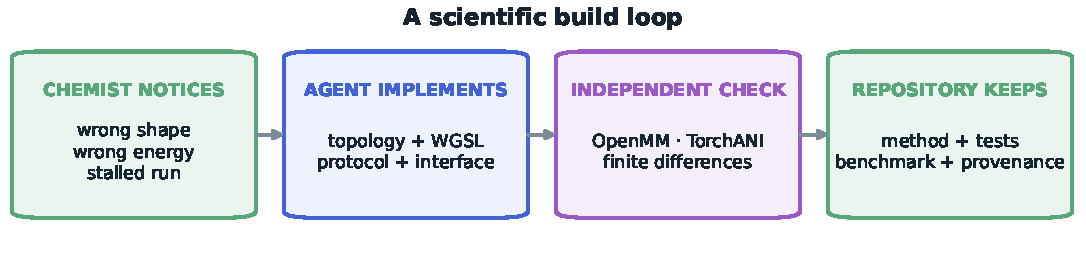
\includegraphics[width=0.94\linewidth]{figures/development-loop.pdf}
  \caption{The development conversation became a repeatable scientific loop.
  Visual and numerical failures produced code changes; independent oracles
  decided whether those changes survived; accepted methods remained with their
  tests and provenance.}
  \label{fig:development-loop}
\end{figure}

That history gives ``free'' four distinct meanings:

\begin{center}
\fcolorbox{MolariumGreen}{MolariumMint}{%
\begin{minipage}{0.945\linewidth}
\vspace{0.35em}
\begin{minipage}[t]{0.47\linewidth}
\textbf{1. Free to use.} The public artifact has no license fee, and supported
calculations need not upload a structure.

\smallskip
\textbf{3. Free to preserve.} A repository can keep agent-written methods long
enough for other scientists to inspect, test, and improve them.
\end{minipage}\hfill
\begin{minipage}[t]{0.47\linewidth}
\textbf{2. Free to rebuild.} \emph{We now take seriously the possibility that a
sufficiently specified method can be implemented from its paper during a
project, rather than awaited as a product.}

\smallskip
\textbf{4. Free to compose.} One interface and explicit protocols can make
methods plug-and-play for chemists and for agents running reproducible
benchmarks.
\end{minipage}
\vspace{0.35em}
\end{minipage}}
\end{center}

This is different from asking a model to call a fixed toolchain. Orchestration is
right when trusted programs and trained models already exist, as recent
protein-design systems demonstrate~\cite{anthropic-protein,openai-rosalind}.
Accordingly, \molarium{} keeps RDKit, OpenMM, ONNX Runtime, and the official
ANI-2x and OpenFold weights~\cite{rdkit,openmm8,onnxruntime,torchani,ani2x,openfold}.
GPT-5.6 Sol wrote the missing browser-specific
layers. Classical mechanics is unusually amenable to this division: equations,
parameters, units, and reference values can make a new implementation answerable
to independent calculation. A neural architecture alone cannot recreate its
weights or its biological evidence. The model identity, conversation, commits,
and validation outputs are part of the project record~\cite{gpt56sol}.

\section{The experiment as it unfolded}

By the end of the conversation, opening \molarium{} felt less like launching a
suite than picking up one persistent molecular model. The 7KPA complex~\cite{pdb7kpa} in
Figure~\ref{fig:workflow} can be prepared, inspected, edited, and locally relaxed
without leaving its scene. The preparation path resolves alternate locations
and explicit connectivity, repairs supported residue atoms, adds hydrogens, and
keeps a crystallographic water when its geometry supports a ligand--protein
bridge. It does not conceal unresolved chemistry behind a green button.

The continuity is practical, not decorative:
\begin{itemize}
  \setlength{\itemsep}{0pt}
  \setlength{\topsep}{0.2em}
  \item \textcolor{MolariumGreen}{\textbf{View}} keeps chains, ligand, waters,
  contacts, and the selected residue together.
  \item \textcolor{MolariumGreen}{\textbf{Build}} stages bond-order, charge, and
  hydrogen edits before cleanup is allowed to move the structure.
  \item \textcolor{MolariumGreen}{\textbf{Inspect}} returns aligned trajectories
  to the same canvas while preserving the raw coordinates for export.
\end{itemize}

\begin{figure}[H]
  \centering
  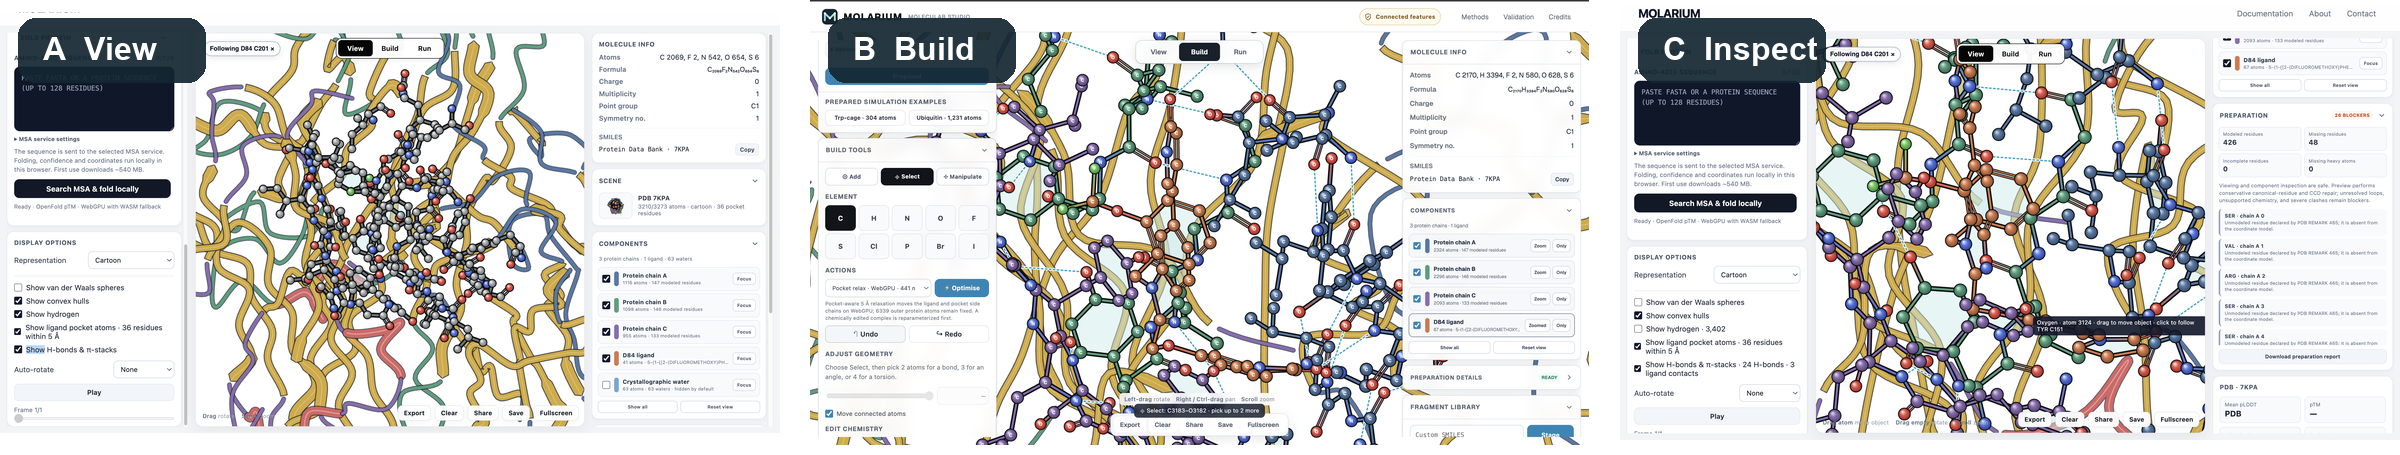
\includegraphics[width=\linewidth]{figures/interface-workflow.png}
  \caption{The same 7KPA protein--ligand system during (A) contact inspection,
  (B) staged chemistry and pocket-local editing, and (C) residue-focused
  inspection. The molecule, selection, and chemical context survive the change
  of task.}
  \label{fig:workflow}
\end{figure}

\section{What the browser had to learn}

The browser is liberating precisely because it refuses the usual assumptions.
There may be no Python, compiler, CUDA driver, or filesystem path that survives
the next machine. WebAssembly gives mature C/C++ code a portable sandbox;
WebGPU gives the page buffers, compute shaders, and command queues, but only fast
f32 arithmetic and no portable 64-bit atomics. The solution was not to pretend
that these constraints did not exist. It was to make them the architecture.

Chemical preparation ends at a numeric System: explicit masses, charges,
bonded terms, Lennard--Jones parameters, exceptions, constraints, and optional
generalized Born parameters. The GPU kernels never guess atom types. Browser
small molecules use OpenFF Sage 2.1; the bundled protein fixtures preserve exact
numeric Systems exported from OpenFF Rosemary 3.0.0-alpha0 with NAGL charges
\cite{sage,rosemary}. From that common boundary, the code chooses a layout that
matches the scientific workload:

\begin{figure}[H]
  \centering
  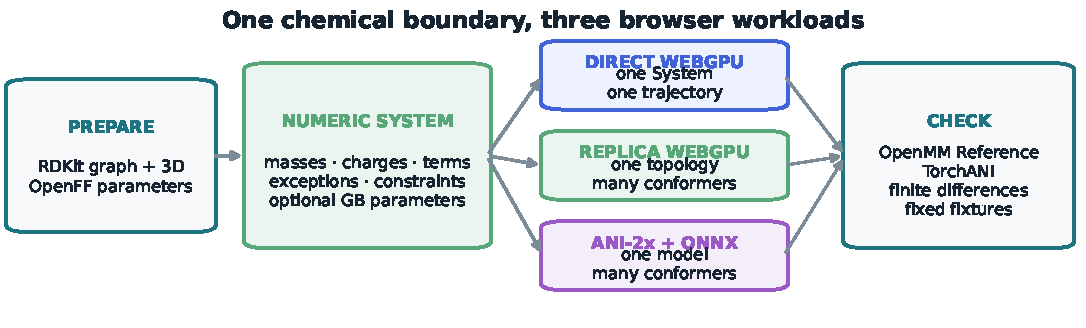
\includegraphics[width=0.94\linewidth]{figures/execution-map.pdf}
  \caption{Preparation stops at an explicit numeric System. Three local
  execution layouts consume it or its coordinates, and each has a deliberately
  separate reference path.}
  \label{fig:execution-map}
\end{figure}

\begin{itemize}
  \setlength{\itemsep}{0.22em}
  \setlength{\topsep}{0.2em}
  \item \textcolor{MolariumGreen}{\textbf{One System, one trajectory.}}
  Atom-centric WGSL kernels evaluate analytic Sage valence, Coulomb,
  Lennard--Jones, and OBC2/ACE forces from sparse incidence buffers
  \cite{sage,obc2,ace}.
  \item \textcolor{MolariumGreen}{\textbf{One topology, many replicas.}}
  A second engine adds a replica dimension to every kernel, borrowing STORMM's
  synthesis idea rather than its source code~\cite{stormm}. Split-int64 force
  accumulation and fixed-point coordinates replace missing 64-bit atomics;
  replica-local SHAKE/RATTLE permits a 2 fs Langevin step~\cite{shake,rattle}.
  \item \textcolor{MolariumGreen}{\textbf{One model, many conformers.}}
  WGSL constructs ANI-2x atomic environment vectors, ONNX Runtime evaluates the
  official eight TorchANI networks, and WGSL contracts derivatives back to
  coordinate forces without a CPU round trip~\cite{torchani,ani2x,onnxruntime}.
\end{itemize}

Each path has a deliberately narrow contract. The replica engine accepts
homogeneous topologies, nonperiodic implicit solvent, and no PME; long-time
stability remains to be established. The ANI-2x path is a vacuum model for
neutral, closed-shell molecules of at most 96 supported atoms. OpenFold 2 is the
opposite case: its scientific content is in trained weights, so the browser runs
the existing model locally rather than claiming to reconstruct it~\cite{openfold}.

\claimbox{Equations can be reconstructed and checked. Trained weights,
parameter sets, and accumulated experimental evidence must be preserved.}

Every fast path answers to slower code. OpenMM 8.2 Reference WebAssembly
re-evaluates the same numeric System in double precision~\cite{openmm8}; native
TorchANI checks ANI; finite differences check forces. Reference code is a test
instrument, not a user-facing fallback. This distinction mattered throughout:
agreement checks arithmetic, but shared parameters do not independently validate
force-field assignment.

\section{The conformer experiment}

Conformer search became the first place where all of these choices met. The
useful result was not one photogenic minimum but a diverse, inspectable set whose
provenance stayed visible.

\claimbox{ETKDGv3 seeds; MMFF94/UFF polish; Sage replica dynamics; common Sage
and ANI scores; symmetry-aware clustering.}

RDKit generates up to 64 symmetry-pruned ETKDGv3 seeds
\cite{rdkit,etkdg,etkdgv3} and briefly polishes them with MMFF94 or UFF
\cite{mmff94,uff}. The replica schedule then applies
2,500 Langevin
steps at 600, 450, and 300 K, followed by 240 fixed-step Sage relaxation
iterations in OBC2/ACE~\cite{sage,obc2,ace}. This final stage is a bounded relaxation, not a converged
minimizer. Symmetry-aware heavy-atom RMSD removes duplicate structures before
clustering and SDF export.

The comparison retains three generators from the same seeds: MMFF-polished
coordinates, replica/Sage coordinates, and ANI-2x-refined coordinates. All final
coordinates receive a common Sage/OBC2 energy and, for supported molecules, a
vacuum ANI-2x energy. The common Sage score makes the generators comparable and
checks replica-engine parity on identical coordinates. It is not an independent
physical oracle: the replica lane optimizes the same objective. The map can plot
energy, structural variables, or rank against rank; color reports the generator,
not the scoring model.

In an eight-molecule development panel, replica search found a lower common
Sage minimum for four molecules. The median best-energy gain was only
0.128 kcal/mol. It added 75 structural clusters, including 44 within 3 kcal/mol
that were absent from the seed lane's window. The current evidence supports
faster exploration and added diversity. It does not establish better conformer
quality in general.

\begin{figure}[H]
  \centering
  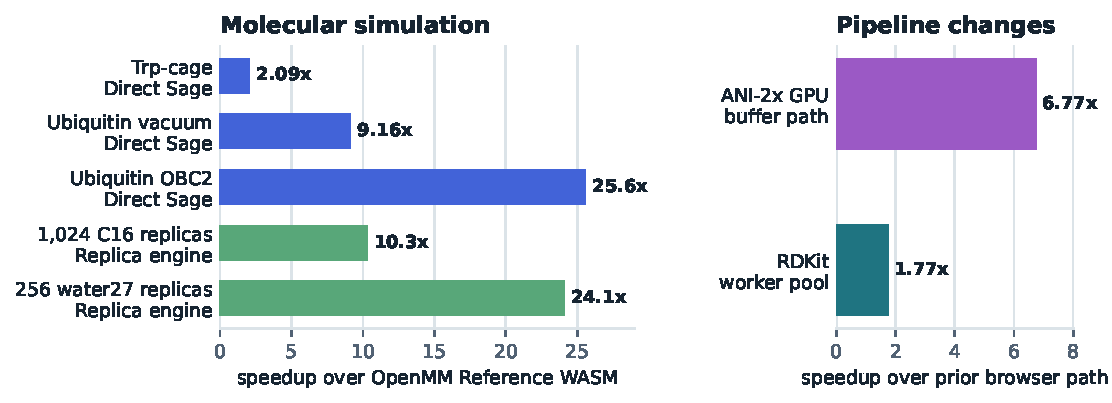
\includegraphics[width=0.48\linewidth]{figures/performance.pdf}
  \caption{Engineering timings on one Apple M1 Pro. Direct and replica
  simulations use OpenMM Reference WebAssembly baselines; replica results omit
  setup and readback and use different integrators. ANI-2x and RDKit compare
  with prior browser paths. None are native-CPU or CUDA comparisons.}
  \label{fig:performance}
\end{figure}

\section{What survived measurement}

The first honest result was negative: a GPU is a poor place to launch one tiny
molecule. OpenMM Reference was 13.3-fold faster for one
C16 and 3.5-fold faster for one water27 because GPU dispatch dominates tiny
jobs. Larger or batched work reversed the result. Direct WebGPU reached
2.09-fold the Reference throughput for 304-atom Trp-cage, 9.16-fold for
1,231-atom vacuum ubiquitin, and 25.6-fold for ubiquitin with OBC2/ACE. At equal
aggregate steps, 1,024 C16 replicas reached 10.3-fold and 256 water27 replicas
24.1-fold the Reference throughput. The baseline is double-precision OpenMM
Reference WebAssembly, not native CPU or CUDA. Replica timings exclude setup and
readback, and the integrators differ.

\claimbox{WebGPU did not make one small molecule fast. It made enough molecular
work fast.}

Numerical tests are separate from product regressions. Direct Sage's largest
relative energy deviation from OpenMM was 2.361e-6; aspirin force relative RMS
was 7.696e-7. Aspirin OBC2 differed by 1.279e-4 kcal/mol with 7.835e-7 force
relative RMS. The replica engine's largest energy error was
2.15e-5 kcal/mol and force relative RMS was 6.66e-6. Against native TorchANI on
six small molecules, ANI-2x reached 0.02572 kcal/mol maximum energy error and
1.022e-5 force relative RMS. These fixtures test implementation parity, not
force-field accuracy, ANI transferability, or cross-vendor agreement.

The 418 browser checks prevent product regressions; they are not 418 scientific
validations. Against prior browser paths, GPU-resident ANI descriptors and
forces improved that stage 6.77-fold, while parallel RDKit workers improved a
cold seed-generation run 1.77-fold (Figure~\ref{fig:performance}).

\section{What this does---and does not---show}

The engines are nonperiodic and omit PME, barostats, membranes, and arbitrary
OpenMM plugins. The single-precision, all-pairs replica engine accepts one
topology at a time. OBC2 and browser protein parameterization remain
experimental; ANI-2x is a restricted vacuum model; OpenFold supports one short
chain and uses a network service only for a user-requested MSA.

Next tests require a frozen conformer benchmark with repeated seeds,
reference-conformer recall, an independent energy judge, confidence intervals,
and a matched modern CPU baseline. The engines also need a cross-GPU matrix and
longer NVE and constrained-solvent trajectories.

The conversation is part of the evidence, not decoration. We are preserving its
timestamped transcript alongside commits, test outputs, benchmark artifacts,
and file hashes, with credentials and private structure data removed before
public release. Until active time is reconstructed from that archive, ``several
days'' denotes the observed project interval rather than a controlled
productivity measurement.

\molarium{} is public at \url{https://molarium.org}; source is at
\url{https://github.com/rafwiewiora/molarium}. We began by asking for a nicer
place to look at molecules. We ended with a sharper proposition: a chemist can
now ask for missing scientific software during the work itself, watch it fail,
demand the relevant comparison, and keep the resulting method as a public,
testable artifact. GPT-5.6 Sol supplied extraordinary implementation speed. The
chemist supplied the taste to notice a flat trifluoromethyl group, the suspicion to question an
energy scale, and the judgment to decide which failure mattered. Neither role is
dispensable. The exciting future is not chemistry without chemists; it is
chemistry in which beautiful ideas no longer have to wait for beautiful tools.

\begin{thebibliography}{24}\fontsize{8}{7.5}\selectfont
\setlength{\itemsep}{-3pt}
\setlength{\parsep}{0pt}

\bibitem{webassembly}
A. Haas et al. WebAssembly. \emph{PLDI} (2017).

\bibitem{webgpu}
W3C GPU for the Web Working Group. \href{https://www.w3.org/TR/webgpu/}{WebGPU
specification}.

\bibitem{ngl}
A. S. Rose and P. W. Hildebrand. NGL Viewer. \emph{Nucleic Acids Research} 43,
W576--W579 (2015).

\bibitem{openmm8}
P. Eastman et al. OpenMM 8. \emph{J. Phys. Chem. B} 128, 109--116 (2024).
\href{https://doi.org/10.1021/acs.jpcb.3c06662}{doi:10.1021/acs.jpcb.3c06662}.

\bibitem{rdkit}
G. Landrum. RDKit: open-source cheminformatics, Release 2025.03.4.
\href{https://doi.org/10.5281/zenodo.591637}{doi:10.5281/zenodo.591637}.

\bibitem{etkdg}
S. Riniker and G. A. Landrum. Better informed distance geometry for conformer
generation. \emph{J. Chem. Inf. Model.} 55, 2562--2574 (2015).
\href{https://doi.org/10.1021/acs.jcim.5b00654}{doi:10.1021/acs.jcim.5b00654}.

\bibitem{etkdgv3}
S. Wang et al. ETKDG conformer generation for small rings and macrocycles.
\emph{J. Chem. Inf. Model.} 60, 2044--2058 (2020).
\href{https://doi.org/10.1021/acs.jcim.0c00025}{doi:10.1021/acs.jcim.0c00025}.

\bibitem{mmff94}
T. A. Halgren. Merck molecular force field I: MMFF94. \emph{J. Comput. Chem.}
17, 490--519 (1996).

\bibitem{uff}
A. K. Rapp\'e et al. UFF. \emph{J. Am. Chem. Soc.} 114, 10024--10035 (1992).
\href{https://doi.org/10.1021/ja00051a040}{doi:10.1021/ja00051a040}.

\bibitem{sage}
S. Boothroyd et al. Open Force Field 2.0.0: Sage. \emph{J. Chem. Theory Comput.}
19, 3251--3275 (2023).
\href{https://doi.org/10.1021/acs.jctc.3c00039}{doi:10.1021/acs.jctc.3c00039}.

\bibitem{obc2}
A. Onufriev, D. Bashford, and D. A. Case. Modified generalized Born model.
\emph{Proteins} 55, 383--394 (2004).
\href{https://doi.org/10.1002/prot.20033}{doi:10.1002/prot.20033}.

\bibitem{ace}
A. Schaefer and M. Karplus. Analytical continuum electrostatics. \emph{J. Phys.
Chem.} 100, 1578--1599 (1996).
\href{https://doi.org/10.1021/jp9521621}{doi:10.1021/jp9521621}.

\bibitem{shake}
J.-P. Ryckaert, G. Ciccotti, and H. J. C. Berendsen. SHAKE constraints.
\emph{J. Comput. Phys.} 23, 327--341 (1977).
\href{https://doi.org/10.1016/0021-9991(77)90098-5}{doi:10.1016/0021-9991(77)90098-5}.

\bibitem{rattle}
H. C. Andersen. RATTLE. \emph{J. Comput. Phys.} 52, 24--34 (1983).
\href{https://doi.org/10.1016/0021-9991(83)90014-1}{doi:10.1016/0021-9991(83)90014-1}.

\bibitem{stormm}
D. S. Cerutti, R. Wiewiora, S. Boothroyd, and W. Sherman. STORMM. \emph{J.
Chem. Phys.} 161, 032501 (2024).
\href{https://doi.org/10.1063/5.0211032}{doi:10.1063/5.0211032}.

\bibitem{torchani}
X. Gao et al. TorchANI. \emph{J. Chem. Inf. Model.} 60, 3408--3415 (2020).
\href{https://doi.org/10.1021/acs.jcim.0c00451}{doi:10.1021/acs.jcim.0c00451}.

\bibitem{ani2x}
C. Devereux et al. ANI-2x: extending ANI to sulfur and halogens. \emph{J. Chem.
Theory Comput.} 16, 4192--4202 (2020).
\href{https://doi.org/10.1021/acs.jctc.0c00121}{doi:10.1021/acs.jctc.0c00121}.

\bibitem{onnxruntime}
Microsoft. \href{https://onnxruntime.ai/}{ONNX Runtime}, Web release 1.27.0.

\bibitem{rosemary}
Open Force Field Initiative. OpenFF Rosemary 3.0.0-alpha0 and NAGL
openff-gnn-am1bcc-1.0.0; exact fixture provenance is archived with
\href{https://github.com/rafwiewiora/molarium/tree/main/openff}{Molarium}.

\bibitem{openfold}
G. Ahdritz et al. OpenFold. \emph{Nature Methods} 21, 1514--1524 (2024).
\href{https://doi.org/10.1038/s41592-024-02272-z}{doi:10.1038/s41592-024-02272-z}.

\bibitem{pdb7kpa}
Protein Data Bank. Structure 7KPA.
\href{https://doi.org/10.2210/pdb7KPA/pdb}{doi:10.2210/pdb7KPA/pdb}.

\bibitem{gpt56sol}
OpenAI. GPT-5.6 Sol. Model-assisted development record, prompts, commits, test
artifacts, and hashes are described in the
\href{https://github.com/rafwiewiora/molarium/blob/main/paper/PROVENANCE-ARCHIVE.md}{Molarium provenance archive} (2026).

\bibitem{anthropic-protein}
Anthropic. \href{https://www.anthropic.com/research/Claude-accelerates-protein-design}{Claude
accelerates protein design} (2026).

\bibitem{openai-rosalind}
OpenAI. \href{https://openai.com/index/introducing-new-capabilities-to-gpt-rosalind/}{Introducing
new capabilities to GPT--Rosalind} (2026).

\end{thebibliography}

\end{document}
